\chapter{रासायनिक मापन की सांख्यिकी}\label{ch:b2:measurement-statistics}

दो प्रयोगशालाएँ एक ही नल के जल में लेड मापती हैं और 9.6 तथा \qty{11.2}{\micro g/L} बताती हैं।
पेयजल के लिए दिशानिर्देश मान \qty{10}{\micro g/L} है। क्या जल पीने योग्य है? क्या दोनों
प्रयोगशालाएँ असहमत भी हैं, या दोनों परिणाम दो मापनों के प्रकीर्णन से होकर देखा गया एक ही मान हैं?
किसी विश्लेषण से मिली संख्या अपनी अनिश्चितता के बिना निरर्थक है, और यह अध्याय उसे परिकलित करने के
साधन देता है: पुनरावृत्त मापनों की सांख्यिकी, किसी परिकलन से होकर अनिश्चितताओं का संचरण,
न्यूनतम वर्गों द्वारा अंशांकन, और वे सीमाएँ जिनके नीचे कोई विधि कुछ नहीं देखती।
% ledger: who:lead

\begin{omfigure}
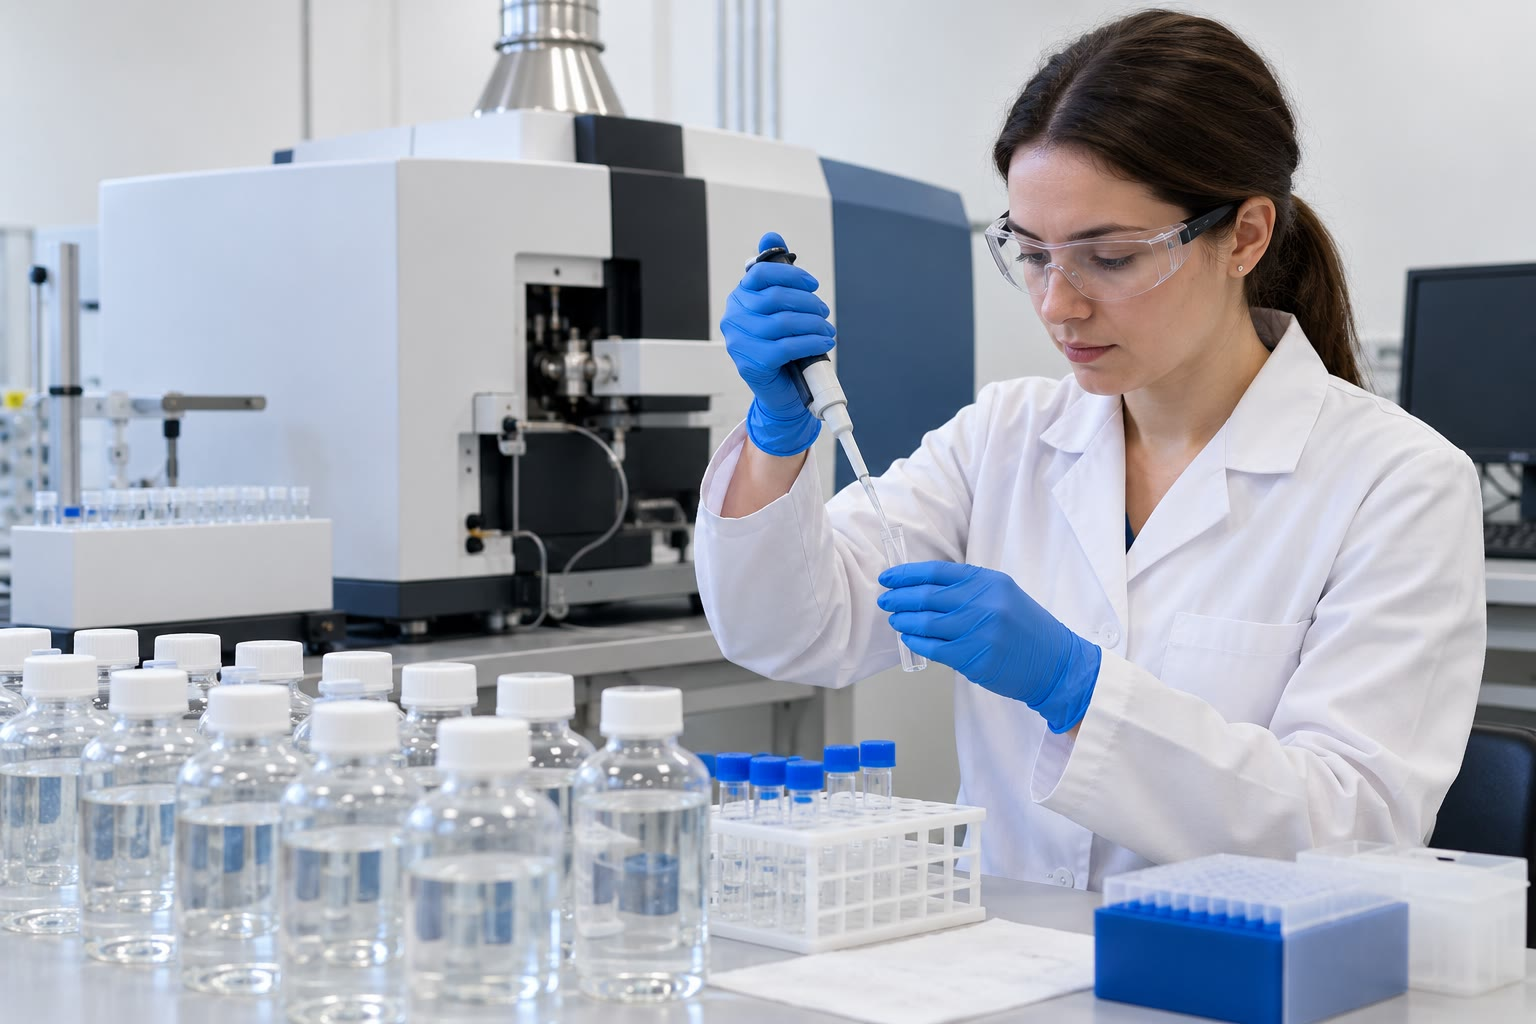
\includegraphics[width=0.56\linewidth]{images/book3/ai/b2-34-water-lab.jpg}

{\small जल-परीक्षण प्रयोगशाला: नमूना बोतलें, पिपेट से मापता एक तकनीशियन, पीछे एक तत्व
विश्लेषक (चित्रण)।}
\end{omfigure}

\begin{recall}
प्रथम वर्ष का खंड: मापन अनिश्चितता, मानक अनिश्चितता, A-प्रकार और B-प्रकार मूल्यांकन,
विस्तारित अनिश्चितता, आपेक्षिक अनिश्चितता, दो मानों के बीच प्रसामान्यीकृत विचलन $z$, और
$u(\bar x) = s/\sqrt n$ तथा एक सामान्य संचरण नियम के प्रमाण का वचन। विद्यालय का खंड:
अंशांकन रेखा। \Cref{ch:b2:mass-spec-atomic}: परमाण्वीय अवशोषण।
\end{recall}

\section{पुनरावृत्त मापन}

किसी मापन को दोहराइए और परिणाम बिखर जाते हैं। हम हर परिणाम $x_i$ को एक यादृच्छिक चर मानते हैं जिसका
माध्य $\mu$ (वह मान जो विधि औसतन देती) और मानक विचलन $\sigma$ है; जब अनेक
छोटे स्वतंत्र कारण जुड़ते हैं, तो परिणाम प्रसामान्य (गाउसीय) नियम का अनुसरण करते हैं, उनमें से लगभग 68~\%
$\mu \pm \sigma$ के भीतर और 95~\% $\mu \pm 1.96\sigma$ के भीतर।

\begin{definition}[प्रकीर्णन]\label{def:b2:measurement-statistics:dispersion}
$n$ परिणामों $x_1, \dots, x_n$ के लिए, जिनका माध्य $\bar x$ है, \emph{प्रायोगिक मानक
विचलन}\index{प्रायोगिक मानक विचलन} $s = \sqrt{\sum (x_i - \bar x)^2/(n-1)}$ है; यह
$\sigma$ का आकलन करता है। \emph{माध्य का मानक विचलन}\index{माध्य का मानक विचलन}
$\bar x$ का मानक विचलन है, $n$ परिणामों की अनेक श्रृंखलाओं पर, जिसका आकलन $s/\sqrt n$ से होता है।
\end{definition}

भाजक $n - 1$, न कि $n$, इस तथ्य को सुधारता है कि विचलन $\bar x$ से लिए गए हैं,
जो स्वयं उन्हीं आँकड़ों से परिकलित है, जिससे वे थोड़े बहुत छोटे हो जाते हैं: $n - 1$
स्वतंत्र विचलनों की संख्या है, अर्थात् स्वातंत्र्य कोटियाँ।

\begin{theorem}[माध्य का प्रसरण]\label{thm:b2:measurement-statistics:mean-variance}
यदि $x_1, \dots, x_n$ स्वतंत्र हैं, जिनमें से हर एक का प्रसरण $\sigma^2$ है, तो $\operatorname{var}(\bar x) =
\sigma^2/n$: \omterm{def:b2:measurement-statistics:dispersion}{माध्य का मानक विचलन} $\sigma/\sqrt n$ है।
\end{theorem}

\begin{proof}
स्वतंत्र चरों के लिए किसी योग का प्रसरण प्रसरणों का योग है, और
$\operatorname{var}(cX) = c^2\operatorname{var}(X)$। अतः $\operatorname{var}(\bar x) =
\operatorname{var}\bigl(\tfrac1n\sum x_i\bigr) = \tfrac{1}{n^2}\sum\operatorname{var}(x_i) =
\tfrac{1}{n^2}\,n\sigma^2 = \sigma^2/n$। $\sigma$ के स्थान पर उसका आकलन $s$ रखने से प्रथम वर्ष के खंड में स्वीकृत
A-प्रकार मानक अनिश्चितता $u(\bar x) = s/\sqrt n$ मिलती है।
\end{proof}

\section{विश्वास्यता अंतराल}

\begin{definition}[विश्वास्यता अंतराल]\label{def:b2:measurement-statistics:confidence}
\emph{विश्वास्यता स्तर}\index{विश्वास्यता स्तर}
$1 - \alpha$ (प्रायः 95~\%) पर \emph{विश्वास्यता अंतराल}\index{विश्वास्यता अंतराल} आँकड़ों से किसी ऐसे नियम द्वारा परिकलित अंतराल है जो,
अनेक श्रृंखलाओं पर लागू होने पर, उनके अंश $1 - \alpha$ में वास्तविक मान को समाविष्ट करता है। $n$ परिणामों के माध्य के लिए यह
$\bar x \pm t\,s/\sqrt n$ है, जहाँ $t$ $n - 1$ स्वातंत्र्य कोटियों और उस स्तर के लिए
\emph{स्टूडेंट गुणांक}\index{स्टूडेंट गुणांक} है।
\end{definition}

\begin{proposition}[स्टूडेंट नियम]\label{prop:b2:measurement-statistics:student}
$n$ स्वतंत्र प्रसामान्य परिणामों के लिए $T = (\bar x - \mu)/(s/\sqrt n)$
$n - 1$ स्वातंत्र्य कोटियों वाले स्टूडेंट नियम का अनुसरण करता है, जिसका घनत्व $(1 + t^2/\nu)^{-(\nu+1)/2}$ के समानुपाती है,
$\nu = n - 1$ के साथ। यह प्रसामान्य नियम से चौड़ा है और $n$ के बढ़ने पर उसकी ओर प्रवृत्त होता है।
\end{proposition}

\admitted

$s$ से भाग देने से, अज्ञात $\sigma$ के बजाय, स्वयं $s$ का प्रकीर्णन जुड़ जाता है, जो $n$ के
छोटे होने पर बड़ा होता है; इसीलिए भारी पुच्छ, और 1.96 से बड़े गुणांक। सारणी 95~\% वाले
गुणांक देती है, जो घनत्व से परिकलित हैं।

\begin{omfigure}
\begin{minipage}[c]{0.56\linewidth}
\begin{tikzpicture}
\begin{axis}[width=\linewidth, height=4.8cm, xmin=-5, xmax=5, ymin=0, ymax=0.43,
  xlabel={$t$}, ylabel={घनत्व}, label style={font=\small}, tick label style={font=\scriptsize},
  legend style={font=\scriptsize, at={(0.98,0.98)}, anchor=north east}, legend cell align=left]
\addplot[omThm, thick] table[x=t, y=nu2] {figdata/out/bachelor-2-regression-c.dat};
\addplot[omMeth, thick] table[x=t, y=nu5] {figdata/out/bachelor-2-regression-c.dat};
\addplot[black, thick, dashed] table[x=t, y=normal] {figdata/out/bachelor-2-regression-c.dat};
\legend{$\nu = 2$, $\nu = 5$, प्रसामान्य}
\end{axis}
\end{tikzpicture}
\end{minipage}\hfill
\begin{minipage}[c]{0.4\linewidth}\centering
\small
\begin{tabular}{rr}
\hline
$\nu = n - 1$ & $t$ (95~\%) \\
\hline
1 & 12.706 \\
2 & 4.303 \\
3 & 3.182 \\
4 & 2.776 \\
5 & 2.571 \\
9 & 2.262 \\
20 & 2.086 \\
$\infty$ & 1.960 \\
\hline
\end{tabular}
\end{minipage}
\par\vspace{4pt}

{\small प्रसामान्य नियम की तुलना में 2 और 5 स्वातंत्र्य कोटियों के स्टूडेंट घनत्व, और द्वि-पक्षीय
95~\% गुणांक, घनत्व के समाकलन से परिकलित (अंतिम पंक्ति प्रसामान्य नियम है)।}
% figdata: bachelor-2/regression.py parts c, e
\end{omfigure}

\begin{method}[किसी माध्य के लिए विश्वास्यता अंतराल]\label{met:b2:measurement-statistics:confidence-interval}
\begin{enumerate}
  \item $\bar x$ और $s$ परिकलित कीजिए, $n$ परिणामों के; जाँचिए कि कोई परिणाम बहुत अलग न हो।
  \item $t$ पढ़िए, $\nu = n - 1$ के लिए, चुने गए स्तर पर।
  \item $\bar x \pm t\,s/\sqrt n$ बताइए, अनिश्चितता को एक या दो सार्थक अंकों तक पूर्णांकित करके
        और माध्य को उसी दशमलव स्थान तक।
  \item किसी संदर्भ मान $x_{\mathrm{ref}}$ से तुलना के लिए $|\bar x - x_{\mathrm{ref}}|/(s/\sqrt
        n)$ परिकलित कीजिए: $t$ से ऊपर होने पर अंतर उस स्तर पर सार्थक है; नीचे होने पर आँकड़े कोई
        अंतर नहीं दिखाते (जो यह सिद्ध नहीं करता कि अंतर है ही नहीं)।
\end{enumerate}
\end{method}

\section{अनिश्चितता का संचरण}

\begin{theorem}[अनिश्चितता संचरण का नियम]\label{thm:b2:measurement-statistics:propagation}
यदि $y = f(x_1, \dots, x_n)$, जहाँ $x_i$ स्वतंत्र हैं और उनकी मानक अनिश्चितताएँ $u(x_i)$ इतनी छोटी हैं
कि उन पर $f$ लगभग रैखिक हो, तो
\begin{equation*}
u^2(y) = \sum_{i=1}^{n}\left(\frac{\partial f}{\partial x_i}\right)^2 u^2(x_i).
\end{equation*}
\end{theorem}

\begin{proof}
प्रथम कोटि तक (टेलर), $y - f(\mu_1, \dots, \mu_n) \approx \sum c_i(x_i - \mu_i)$, जहाँ $c_i = \partial
f/\partial x_i$ माध्यों पर। स्वतंत्र चरों के किसी रैखिक संयोजन का प्रसरण
$\sum c_i^2\operatorname{var}(x_i)$ है (जैसे \cref{thm:b2:measurement-statistics:mean-variance} में);
$\operatorname{var}(x_i) = u^2(x_i)$ के साथ यही परिणाम है।
\end{proof}

\begin{corollary}[योग और गुणनफल]\label{cor:b2:measurement-statistics:products}
किसी योग या अंतर के लिए मानक अनिश्चितताएँ वर्ग-योग में जुड़ती हैं: $u^2(x_1 \pm x_2) = u^2(x_1) +
u^2(x_2)$। किसी गुणनफल या भागफल $y = x_1^{a}x_2^{b}\cdots$ के लिए आपेक्षिक अनिश्चितताएँ
वर्ग-योग में जुड़ती हैं, हर एक अपने घातांक से भारित: $\bigl(u(y)/y\bigr)^2 = a^2\bigl(u(x_1)/x_1\bigr)^2 +
b^2\bigl(u(x_2)/x_2\bigr)^2 + \cdots$
\end{corollary}

\begin{proof}
योग के लिए आंशिक अवकलज $\pm1$ हैं। $y = x_1^ax_2^b$ के लिए $\partial y/\partial x_1 =
a\,y/x_1$ और $\partial y/\partial x_2 = b\,y/x_2$; प्रमेय $u^2(y) = a^2y^2u^2(x_1)/x_1^2 +
b^2y^2u^2(x_2)/x_2^2$ देता है; $y^2$ से भाग दीजिए।
\end{proof}

\begin{method}[संचरण]\label{met:b2:measurement-statistics:propagate}
\begin{enumerate}
  \item परिणाम को मापी गई राशियों के सूत्र के रूप में लिखिए; हर निवेश को उसकी मानक
        अनिश्चितता (A या B प्रकार) के साथ सूचीबद्ध कीजिए।
  \item गुणनफलों और भागफलों के लिए आपेक्षिक अनिश्चितताओं से काम कीजिए; योगों के लिए निरपेक्ष से;
        अन्यथा आंशिक अवकलज लीजिए।
  \item वर्ग-योग में संयोजित कीजिए; प्रभावी पद खोजिए: बाक़ी को सुधारना व्यर्थ प्रयास है।
  \item विस्तारित अनिश्चितता के लिए आवरण गुणक (2, या स्टूडेंट $t$ जब प्रभावी पद कम
        पुनरावृत्तियों से आता हो) से गुणा कीजिए।
\end{enumerate}
\end{method}

\section{अंशांकन}

\begin{definition}[अंशांकन वक्र]\label{def:b2:measurement-statistics:calibration}
\emph{अंशांकन वक्र}\index{अंशांकन वक्र} किसी उपकरण के संकेत $y$ को
सांद्रता $x$ से संबंधित करता है, ज्ञात सांद्रता वाले मानकों से। \emph{न्यूनतम-वर्ग
रेखा}\index{न्यूनतम-वर्ग रेखा} $y = a + bx$ वह रेखा है जो $S = \sum (y_i - a -
bx_i)^2$ को न्यूनतम करती है; हर $e_i = y_i - a - bx_i$ एक \emph{अवशिष्ट}\index{अवशिष्ट} है।
\end{definition}

\begin{theorem}[न्यूनतम-वर्ग रेखा]\label{thm:b2:measurement-statistics:least-squares}
माध्यों $\bar x$, $\bar y$, $S_{xx} = \sum(x_i - \bar x)^2$ और $S_{xy} = \sum(x_i - \bar x)(y_i -
\bar y)$ के साथ \omterm{def:b2:measurement-statistics:calibration}{न्यूनतम-वर्ग रेखा} के लिए
\begin{equation*}
b = \frac{S_{xy}}{S_{xx}}, \qquad a = \bar y - b\bar x.
\end{equation*}
\end{theorem}

\begin{proof}
$S$, $a$ और $b$ का एक द्विघाती फलन है। न्यूनतम पर इसके आंशिक अवकलज शून्य होते हैं:
$\partial S/\partial a = -2\sum(y_i - a - bx_i) = 0$ से $a = \bar y - b\bar x$ मिलता है; इसे
$\partial S/\partial b = -2\sum x_i(y_i - a - bx_i) = 0$ में रखने पर $\sum x_i\bigl((y_i - \bar y) - b(x_i -
\bar x)\bigr) = 0$ मिलता है, अर्थात् $S_{xy} = bS_{xx}$ (क्योंकि $\sum \bar x(y_i - \bar y) = \sum \bar x(x_i - \bar
x) = 0$)। द्वितीय अवकलज यह आव्यूह बनाते हैं:
\[\begin{pmatrix} 2n & 2\sum x_i\\ 2\sum x_i & 2\sum x_i^2\end{pmatrix},\]
जिसका विकर्ण धनात्मक है और जिसका सारणिक $4nS_{xx}$ धनात्मक है जब सभी $x_i$
समान न हों: स्तब्ध बिंदु एक न्यूनतम है।
\end{proof}

\begin{proposition}[सांद्रता पढ़ना]\label{prop:b2:measurement-statistics:interpolation}
$n$ मानकों के लिए, जिनका \omterm{def:b2:measurement-statistics:calibration}{अवशिष्ट} मानक विचलन $s_{y/x} = \sqrt{\sum e_i^2/(n-2)}$ है, कोई नमूना जिसे
$m$ बार पढ़ा गया हो और जिसका माध्य संकेत $\bar y_0$ हो, उसके लिए $x_0 = (\bar y_0 - a)/b$ और मानक विचलन यह है:
\begin{equation*}
s_{x_0} = \frac{s_{y/x}}{b}\sqrt{\frac1m + \frac1n + \frac{(\bar y_0 - \bar y)^2}{b^2S_{xx}}},
\end{equation*}
जिसे स्टूडेंट $t$ के साथ, $n - 2$ स्वातंत्र्य कोटियों के लिए, प्रयुक्त करना है।
\end{proposition}

\admitted

मूल के नीचे के तीनों पद नमूना पाठ्यांकों का प्रकीर्णन, रेखा की ऊँचाई की अनिश्चितता और
उसकी ढाल की अनिश्चितता हैं; अंतिम पद अंशांकन परास के केंद्र पर शून्य हो जाता है, जहाँ
नमूने सबसे अच्छे पढ़े जाते हैं।

\begin{omfigure}
\begin{tikzpicture}
\begin{axis}[width=0.5\linewidth, height=5cm, xmin=-1, xmax=22, ymin=0, ymax=0.22,
  xlabel={लेड (\unit{\micro g/L})}, ylabel={अवशोषकता}, label style={font=\small},
  tick label style={font=\scriptsize}, scaled y ticks=false,
  yticklabel style={/pgf/number format/fixed, /pgf/number format/precision=2}]
\addplot[omDef, thick] table[x=x, y=line] {figdata/out/bachelor-2-regression-b.dat};
\addplot[only marks, mark=*, mark size=1.8pt, omThm] table[x=x, y=A] {figdata/out/bachelor-2-regression-a.dat};
\end{axis}
\end{tikzpicture}\hfill
\begin{tikzpicture}
\begin{axis}[width=0.5\linewidth, height=5cm, xmin=-1, xmax=22, ymin=-0.002, ymax=0.002,
  xlabel={लेड (\unit{\micro g/L})}, ylabel={अवशिष्ट}, label style={font=\small},
  tick label style={font=\scriptsize}, scaled y ticks=false, ycomb,
  yticklabel style={/pgf/number format/fixed, /pgf/number format/precision=3},
  extra y ticks={0}, extra y tick style={grid=major, grid style={black!50}}]
\addplot[omThm, thick, mark=*, mark size=1.6pt] table[x=x, y=res] {figdata/out/bachelor-2-regression-a.dat};
\end{axis}
\end{tikzpicture}

{\small \qty{283.3}{nm} पर ग्रेफ़ाइट-भट्टी परमाण्वीय अवशोषण द्वारा लेड का अंशांकन (अभ्यास के आँकड़े,
समस्या में प्रयुक्त)। बाएँ: पाँच मानक और \omterm{def:b2:measurement-statistics:calibration}{न्यूनतम-वर्ग रेखा}। दाएँ: \omterm{def:b2:measurement-statistics:calibration}{अवशिष्ट}, छोटे
और बिना किसी पैटर्न के: सरल रेखा पर्याप्त है।}
% figdata: bachelor-2/regression.py parts a, b
% ledger: asd:Pb283
\end{omfigure}

\begin{method}[अंशांकन]\label{met:b2:measurement-statistics:calibrate}
\begin{enumerate}
  \item अपेक्षित परास को फैलाने वाले पाँच या अधिक मानक, नमूनों जैसी ही आधात्री में,
        और एक रिक्त बनाइए।
  \item \omterm{def:b2:measurement-statistics:calibration}{न्यूनतम-वर्ग रेखा} समंजित कीजिए; \omterm{def:b2:measurement-statistics:calibration}{अवशिष्ट} आलेखित कीजिए। वक्र पैटर्न का अर्थ है कि अनुक्रिया
        रैखिक नहीं है: परास संकरा कीजिए या वक्र समंजित कीजिए। एक बड़ा \omterm{def:b2:measurement-statistics:calibration}{अवशिष्ट} किसी दोषपूर्ण मानक की ओर संकेत करता है।
  \item नमूनों को, अधिमानतः परास के मध्य के निकट, पुनरावृत्ति में पढ़िए; $x_0$ और
        $s_{x_0}$ परिकलित कीजिए।
  \item हर तनुकरण के लिए संशोधन करके $x_0 \pm t\,s_{x_0}$ बताइए, और यदि तनुकरण की संचरित अनिश्चितता
        नगण्य न हो तो उसे जोड़िए।
\end{enumerate}
\end{method}

\begin{definition}[मानक योग]\label{def:b2:measurement-statistics:standard-addition}
\emph{मानक-योग विधि}\index{मानक-योग विधि} में विश्लेष्य की ज्ञात मात्राएँ
स्वयं नमूने के समान भागों में मिलाई जाती हैं; संकेत को मिलाई गई सांद्रता के विरुद्ध आलेखित किया जाता है,
और नमूने में विश्लेष्य की सांद्रता मूल-बिंदु से उस बिंदु तक की दूरी है जहाँ
शून्य संकेत तक बहिर्वेशित रेखा अक्ष को काटती है, $a/b$।
\end{definition}

\begin{method}[मानक योग]\label{met:b2:measurement-statistics:standard-addition}
\begin{enumerate}
  \item इसे तब प्रयुक्त कीजिए जब नमूने की आधात्री अनुक्रिया को बदल दे (लवण, अम्ल, कार्बनिक पदार्थ), जिससे
        शुद्ध जल में बने मानक ग़लत ढाल देते।
  \item समान भागों में बढ़ती ज्ञात मात्राएँ मिलाइए, सभी को समान आयतन तक तनु कीजिए, मापिए।
  \item रेखा समंजित कीजिए; मापे गए विलयनों में सांद्रता $a/b$ है; तनुकरण के लिए संशोधन कीजिए।
  \item अनुक्रिया शून्य से ही रैखिक होनी चाहिए: \omterm{def:b2:measurement-statistics:calibration}{अवशिष्ट} जाँचिए।
\end{enumerate}
\end{method}

\begin{omfigure}
\begin{tikzpicture}
\begin{axis}[width=0.62\linewidth, height=5cm, xmin=-4, xmax=7, ymin=0, ymax=0.42,
  xlabel={मिलाई गई सांद्रता (\unit{mg/L})}, ylabel={अवशोषकता}, label style={font=\small},
  tick label style={font=\scriptsize}, axis lines=left, scaled y ticks=false,
  yticklabel style={/pgf/number format/fixed, /pgf/number format/precision=1}]
\draw[black!40] (axis cs:0,0) -- (axis cs:0,0.42);
\addplot[omDef, thick, densely dashed] table[x=x, y=line] {figdata/out/bachelor-2-regression-d-line.dat};
\addplot[only marks, mark=*, mark size=1.8pt, omThm] table[x=x, y=A] {figdata/out/bachelor-2-regression-d.dat};
\draw[<->, omMeth, thick] (axis cs:-3.11,0.06) -- (axis cs:0,0.06); \node[omMeth, below, font=\scriptsize] at (axis cs:-0.8,0.055) {$a/b$};
\end{axis}
\end{tikzpicture}

{\small मानक योग (अभ्यास के आँकड़े): विश्लेष्य के 0, 2, 4 और
\qty{6}{mg/L} मिलाए गए एक नमूने की अवशोषकता। रेखा \qty{-3.11}{mg/L} पर शून्य संकेत से मिलती है: मापे गए विलयन में
\qty{3.11}{mg/L} था।}
% figdata: bachelor-2/regression.py part d
\end{omfigure}

\section{संसूचन, मात्रांकन और मान्यकरण}

\begin{definition}[सीमाएँ]\label{def:b2:measurement-statistics:limits}
किसी विधि की \emph{संसूचन सीमा}\index{संसूचन सीमा} वह सबसे छोटी सांद्रता है जिसका
संकेत किसी रिक्त के संकेत से, मिथ्या संसूचन के एक बताए गए छोटे जोखिम के साथ, अलग पहचाना जा सके;
\emph{मात्रांकन सीमा}\index{मात्रांकन सीमा} वह सबसे छोटी सांद्रता है जिसे
स्वीकार्य आपेक्षिक अनिश्चितता के साथ मापा जा सके।
\end{definition}

\begin{proposition}[सामान्य आकलन]\label{prop:b2:measurement-statistics:lod}
पुनरावृत्त रिक्त संकेतों के मानक विचलन $s_{\mathrm{blank}}$ और
अंशांकन रेखा की ढाल $b$ के साथ, $x_{\mathrm{LOD}} \approx 3s_{\mathrm{blank}}/b$ और $x_{\mathrm{LOQ}} \approx
10s_{\mathrm{blank}}/b$।
\end{proposition}

\begin{proof}[तर्क]
यदि रिक्त संकेत मानक विचलन $s_{\mathrm{blank}}$ के साथ प्रसामान्य हैं, तो कोई रिक्त अपने माध्य से
$3s_{\mathrm{blank}}$ से अधिक लगभग 0.13~\% प्रायिकता से बढ़ता है (3 मानक विचलनों से आगे प्रसामान्य नियम की
एक-पक्षीय पुच्छ): उस देहली से ऊपर किसी संकेत को ``संसूचित'' कहना शायद ही कभी किसी रिक्त को
नमूना समझने की भूल करता है। रिक्त से $10s_{\mathrm{blank}}$ ऊपर के संकेत का आपेक्षिक मानक विचलन लगभग
10~\% होता है, जो मात्रात्मक परिणाम की सामान्य देहली है। $b$ से भाग देने पर संकेत
सांद्रताओं में बदल जाते हैं।
\end{proof}

\begin{definition}[मान्यकरण]\label{def:b2:measurement-statistics:validation}
\emph{यथार्थता}\index{यथार्थता} बड़ी संख्या में परिणामों के माध्य की वास्तविक
मान से निकटता है; उनका अंतर \emph{अभिनति}\index{अभिनति} है। \emph{परिशुद्धता}\index{परिशुद्धता}
स्वतंत्र परिणामों की एक-दूसरे से निकटता है, जो मानक विचलन के रूप में व्यक्त होती है:
समान परिस्थितियों (वही प्रचालक, उपकरण,
प्रयोगशाला, कम समय) में \emph{पुनरावर्तनीयता}\index{पुनरावर्तनीयता}, बदली हुई परिस्थितियों
(भिन्न प्रयोगशालाएँ) में \emph{पुनरुत्पादनीयता}\index{पुनरुत्पादनीयता}। \emph{विधि मान्यकरण}\index{विधि मान्यकरण} उन प्रयोगों का समुच्चय है
जो किसी विधि के लिए उसकी यथार्थता, परिशुद्धता, रैखिकता और परास, तथा उसकी संसूचन
और मात्रांकन सीमाएँ स्थापित करते हैं।
\end{definition}

\omterm{def:b2:measurement-statistics:validation}{यथार्थता} किसी प्रमाणित संदर्भ पदार्थ के विरुद्ध या ज्ञात मात्रा मिलाकर जाँची जाती है; \omterm{def:b2:measurement-statistics:validation}{परिशुद्धता}
एक प्रयोगशाला में पुनरावृत्तियों से और प्रयोगशालाओं के बीच तुलनाओं से। कोई विधि परिशुद्ध परंतु अभिनत हो सकती है, हर
परिणाम दूसरों के निकट और सभी ग़लत: \omterm{def:b2:measurement-statistics:validation}{परिशुद्धता} \omterm{def:b2:measurement-statistics:validation}{यथार्थता} का प्रमाण नहीं है।

\begin{history}[स्टूडेंट, 1908]
\begin{minipage}[t]{0.17\linewidth}
\vspace{0pt}
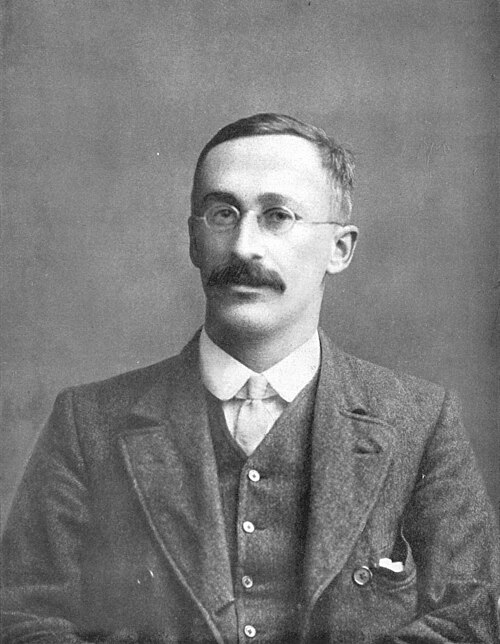
\includegraphics[width=\linewidth]{images/book3/gosset.jpg}
\end{minipage}\hfill
\begin{minipage}[t]{0.79\linewidth}
\vspace{0pt}
विलियम सीली गॉसेट, एक मद्यनिर्माणशाला में काम करने वाले रसायनज्ञ, को बहुत कम नमूनों से कच्चे माल को परखना पड़ता था,
जो प्रसामान्य नियम के लिए बहुत कम थे। 1908 में उन्होंने माध्य को नमूना
मानक विचलन से भाग देने पर मिलने वाला वितरण प्रकाशित किया, छद्म नाम ``स्टूडेंट'' से, क्योंकि उनका नियोक्ता कर्मचारियों को
अपने नाम से प्रकाशन की अनुमति नहीं देता था। जब भी कोई विश्लेषक तीन या चार
पुनरावृत्तियों से कोई अंतराल बताता है, स्टूडेंट नियम प्रयुक्त होता है। (छायाचित्र, 1908: सार्वजनिक अधिकार-क्षेत्र; विकिमीडिया कॉमन्स।)
\end{minipage}
\end{history}

\section{अभ्यास}

\begin{exercise}[$\star$]\label{exo:b2:measurement-statistics:1}
पाँच अनुमापन 12.45, 12.50, 12.48, 12.52 और \qty{12.46}{mL} देते हैं। माध्य,
\omterm{def:b2:measurement-statistics:dispersion}{प्रायोगिक मानक विचलन} और \omterm{def:b2:measurement-statistics:dispersion}{माध्य का मानक विचलन} परिकलित कीजिए।
\end{exercise}

\begin{exercise}[$\star$]\label{exo:b2:measurement-statistics:2}
अभ्यास~1 के माध्य का 95~\% \omterm{def:b2:measurement-statistics:confidence}{विश्वास्यता अंतराल} दीजिए।
\end{exercise}

\begin{exercise}[$\star$]\label{exo:b2:measurement-statistics:3}
किसी ठोस के $m = \qty{0.5000}{g}$ ($u = \qty{0.0002}{g}$) को
$V = \qty{250.0}{mL}$ ($u = \qty{0.15}{mL}$) के फ़्लास्क में घोलकर एक विलयन बनाया जाता है। $c = m/(MV)$ की आपेक्षिक मानक अनिश्चितता परिकलित कीजिए,
मोलर द्रव्यमान को पर्याप्त यथातथ मानते हुए।
\end{exercise}

\begin{exercise}[$\star$]\label{exo:b2:measurement-statistics:4}
$(0, 0.02)$, $(1, 0.21)$, $(2, 0.39)$, $(3, 0.62)$ से होकर \omterm{def:b2:measurement-statistics:calibration}{न्यूनतम-वर्ग रेखा} समंजित कीजिए।
\end{exercise}

\begin{exercise}[$\star\star$]\label{exo:b2:measurement-statistics:5}
किसी प्रमाणित संदर्भ विलयन में किसी तत्व का \qty{10.00}{mg/L} है। पाँच विश्लेषण
$s = \qty{0.08}{mg/L}$ के साथ \qty{10.12}{mg/L} का माध्य देते हैं। क्या 95~\% स्तर पर विधि अभिनत है?
\end{exercise}

\begin{exercise}[$\star\star$]\label{exo:b2:measurement-statistics:6}
हाइड्रोनियम आयनों की सांद्रता 2~\% की आपेक्षिक मानक अनिश्चितता के साथ ज्ञात है। pH की
मानक अनिश्चितता क्या है?
\end{exercise}

\begin{exercise}[$\star\star$]\label{exo:b2:measurement-statistics:7}
दस रिक्तों का $s = 0.0012$ अवशोषकता इकाई है; अंशांकन ढाल \qty{0.0098}{L/\micro g} है।
संसूचन और मात्रांकन की सीमाओं का आकलन कीजिए।
\end{exercise}

\begin{exercise}[$\star\star$]\label{exo:b2:measurement-statistics:8}
चित्र के मानक-योग प्रयोग में चारों भाग नमूने के \qty{10.0}{mL} को
\qty{50.0}{mL} तक तनु करके बनाए गए थे। नमूने में सांद्रता दीजिए।
\end{exercise}

\begin{exercise}[$\star\star$]\label{exo:b2:measurement-statistics:9}
एक अंतर-प्रयोगशाला अध्ययन में हर प्रयोगशाला अपनी पुनरावृत्तियों पर $s = \qty{0.05}{mg/L}$ पाती है, परंतु
भिन्न प्रयोगशालाओं के परिणाम $s = \qty{0.15}{mg/L}$ के साथ बिखरते हैं। दोनों राशियों के नाम बताइए और
अंतर समझाइए।
\end{exercise}

\begin{exercise}[$\star\star\star$]\label{exo:b2:measurement-statistics:10}
दिखाइए कि \omterm{def:b2:measurement-statistics:calibration}{न्यूनतम-वर्ग रेखा} $(\bar x, \bar y)$ से होकर जाती है और उसके \omterm{def:b2:measurement-statistics:calibration}{अवशिष्टों} का योग शून्य है।
\end{exercise}

\begin{exercise}[$\star\star\star$]\label{exo:b2:measurement-statistics:11}
किसी स्टॉक विलयन को सौ गुना तनु किया जाता है, या तो एक चरण में (\qty{1.000}{mL} को \qty{100.0}{mL} में) या
दो दस-गुना चरणों में (\qty{10.00}{mL} को \qty{100.0}{mL} में, दो बार)। मानक अनिश्चितताएँ: 1 mL
पिपेट \qty{0.006}{mL}, 10 mL पिपेट \qty{0.02}{mL}, 100 mL फ़्लास्क \qty{0.08}{mL} (अभ्यास के आँकड़े)।
कौन-सा मार्ग अधिक परिशुद्ध है?
\end{exercise}

\begin{exercise}[$\star\star\star$]\label{exo:b2:measurement-statistics:12}
आरंभ वाली दोनों प्रयोगशालाएँ मानक अनिश्चितताओं 0.4 और \qty{0.5}{\micro g/L} के साथ 9.6 और \qty{11.2}{\micro g/L} बताती हैं
(अभ्यास के आँकड़े)। क्या उनके परिणाम संगत हैं? हर एक दिशानिर्देश मान के बारे में क्या कहता है?
\end{exercise}

\section{समस्या: नल के जल में लेड}

\begin{problem}[{सप्ताहांत समस्या --- न्यूनतम वर्गों द्वारा परमाण्वीय-अवशोषण अंशांकन, किसी नमूने की
सांद्रता उसके विश्वास्यता अंतराल के साथ, तनुकरण और सीमाएँ, और दिशानिर्देश मान के विरुद्ध
निर्णय}]
\label{pb:b2:measurement-statistics:1}
अभ्यास के आँकड़े। लेड को \qty{283.3}{nm} पर ग्रेफ़ाइट-भट्टी परमाण्वीय अवशोषण द्वारा मापा जाता है। मानक
(\unit{\micro g/L}; अवशोषकता): 0.0; 0.003, 5.0; 0.051, 10.0; 0.101, 15.0; 0.148, 20.0; 0.199। नल
के जल (\qty{50.0}{mL}) को नाइट्रिक अम्ल के \qty{0.50}{mL} से अम्लीकृत किया जाता है; इस विलयन के तीन पाठ्यांक
0.104, 0.098 और 0.101 देते हैं। दस रिक्त: 0.002, 0.004, 0.003, 0.001, 0.003, 0.005, 0.002,
0.003, 0.004, 0.003। आयतनों की मानक अनिश्चितताएँ: 50.0 mL के लिए \qty{0.03}{mL},
0.50 mL के लिए \qty{0.005}{mL}। दिशानिर्देश मान: \qty{10}{\micro g/L}।
% ledger: who:lead, asd:Pb283

\medskip
\noindent\textbf{भाग I --- अंशांकन।}
\begin{enumerate}
  \item मानक नमूनों जैसे ही नाइट्रिक अम्ल में क्यों बनाए जाते हैं?
  \item \omterm{def:b2:measurement-statistics:calibration}{न्यूनतम-वर्ग रेखा} की ढाल और अंतःखंड परिकलित कीजिए।
  \item पाँचों \omterm{def:b2:measurement-statistics:calibration}{अवशिष्ट} परिकलित कीजिए।
  \item क्या \omterm{def:b2:measurement-statistics:calibration}{अवशिष्ट} कोई पैटर्न दिखाते हैं? रैखिकता पर निष्कर्ष निकालिए।
  \item $s_{y/x}$ परिकलित कीजिए।
  \item अंतःखंड शून्य क्यों नहीं है?
  \item ढाल क्या मापती है?
\end{enumerate}

\medskip
\noindent\textbf{भाग II --- नमूना।}
\begin{enumerate}[resume]
  \item तीनों पाठ्यांकों का माध्य और मानक विचलन परिकलित कीजिए।
  \item मापे गए विलयन की लेड सांद्रता परिकलित कीजिए।
  \item $s_{x_0}$ परिकलित कीजिए।
  \item कितनी स्वातंत्र्य कोटियाँ, और कौन-सा \omterm{def:b2:measurement-statistics:confidence}{स्टूडेंट गुणांक}?
  \item मापे गए विलयन में सांद्रता का 95~\% अंतराल दीजिए।
  \item नमूने को एक बार के बजाय तीन बार क्यों पढ़ा जाए?
\end{enumerate}

\medskip
\noindent\textbf{भाग III --- तनुकरण और सीमाएँ।}
\begin{enumerate}[resume]
  \item तनुकरण गुणक और नल के जल में सांद्रता परिकलित कीजिए।
  \item दोनों आयतनों की अनिश्चितता को तनुकरण गुणक में संचरित कीजिए।
  \item क्या अंशांकन वाली अनिश्चितता की तुलना में वह अनिश्चितता सार्थक है?
  \item रिक्तों का मानक विचलन और \omterm{def:b2:measurement-statistics:limits}{संसूचन सीमा} परिकलित कीजिए।
  \item \omterm{def:b2:measurement-statistics:limits}{मात्रांकन सीमा} परिकलित कीजिए।
  \item क्या नमूना \omterm{def:b2:measurement-statistics:limits}{मात्रांकन सीमा} से ऊपर है?
\end{enumerate}

\medskip
\noindent\textbf{भाग IV --- निर्णय।}
\begin{enumerate}[resume]
  \item क्या अंतराल में दिशानिर्देश मान समाविष्ट है?
  \item 0.104 का अकेला पाठ्यांक क्या संकेत देता?
  \item यहाँ ``95~\% विश्वास्यता'' का क्या अर्थ है?
  \item प्रयोगशाला अधिक दृढ़ता से निर्णय कैसे कर सकती है?
  \item वह कैसे जाँचेगी कि विधि अभिनत नहीं है?
  \item दिशानिर्देश ``उपचार निष्पादन और विश्लेषणात्मक
        साध्यता के आधार पर'' अनंतिम है। इस समस्या के प्रकाश में दूसरे कारण का क्या अर्थ है?
  \item नल के जल की लेड सांद्रता उसके 95~\% अंतराल के साथ बताइए, और उसकी तुलना
        \qty{10}{\micro g/L} से कीजिए।
\end{enumerate}
\end{problem}
